\chapter{Trasformare un tesauro in un'ontologia}\label{ch3}
\section{Introduzione}
Qui vediamo come sia possibile usare \cduce per creare ontologie a partire da una rappresentazione della conoscenza già formalizzata in altri modi. Per illustrare il processo di creazione faremo riferimento a un esempio facilmente replicabile: la trasformazione di un tesauro in un'ontologia (per una trattazione più astratta e formale sulla re-ingegnerizzazione di un tesauro si veda \cite{re_engineeringThesaurus}). Commenteremo le scelte effettuate e le strategie adottate. L'esempio permette una discussione lineare e senza eccessivi giri di parole mantenendo comunque una buona generalità qualora si applicassero le stesse scelte e strategie a diversi contesti.

Dopo aver trasformato il tesauro in un'ontologia con \cduce, illustriamo brevemente quali altri strumenti avremmo potuto utilizzare, in particolare cercheremo di ottenere risultati analoghi con Protégé discutendo vantaggi e svantaggi di ciascun approccio.

\section{Vantaggi del passaggio da tesauro a ontologia}
Potremmo essere interessati a trasformare un tesauro espresso in SKOS in un'ontologia espressa in OWL per varie ragioni: prima fra tutte, un'ontologia è una rappresentazione più formale della conoscenza e OWL ha un potere espressivo maggiore di SKOS; potremo quindi effettuare Query più avanzate e utilizzare strumenti di inferenza più potenti.

Per presentare questo argomento prendiamo in considerazione il tesauro: \say{Europeana Fashion Thesaurus}\footnote{\url{http://thesaurus.europeanafashion.eu/}} e tentiamo di trasformarlo in un'ontologia. Prima di addentrarci nella parte tecnica forniamo una breve introduzione al tesauro che editeremo.
\subsection{Europeana Fashion Thesaurus: capturing imagination}
L'\say{Europeana Fashion project}\footnote{\url{http://www.europeanafashion.eu/}} è un progetto che si è posto come obbiettivo quello di organizzare sotto una struttura gerarchica tutto ciò che riguardasse la moda, comprendendo anche sinonimi e contrari. Il tesauro si può trovare all'indirizzo: \url{http://thesaurus.europeanafashion.eu/}. Il tesauro permette di accedere in modo logico, organizzato e strutturato a una vasta conoscenza. Data la struttura ad albero le, relazioni tra oggetti sono chiare e l'aggiunta o la ricerca di informazioni può essere fatta in modo rapido ed efficiente.
\subsection{Svantaggi del tesauro}
Per la sua struttura, il tesauro permette una rappresentazione della conoscenza puramente tassonomica; questo in certi contesti può essere una limitazione, ad esempio: nonostante nel tesauro siano presenti sia capi d'abbigliamento che materiali, non c'è nessuna possibilità di mettere in relazione i due concetti in modo formale; inoltre, se avessimo degli strumenti per fare inferenza, non saremmo in grado di dedurre se una bandana è un accessorio per il capo, perché quest'ultima non si trova nel ramo degli accessori della testa.

Il passaggio a un'ontologia permetterebbe di costruire relazioni più complesse per descrivere in modo più ricco gli oggetti del dominio di interesse.
\section{Struttura del tesauro}
La struttura del tesauro che vogliamo re-ingegnerizzare è semplice: in particolare abbiamo una serie di concetti fondamentali da cui partono tutti gli altri rami che rappresentano i concetti derivati. I concetti fondamentali, almeno per quello che ci interessa, sono:
\begin{itemize}
	\item oggetti di moda;
	\item colori;
	\item tecniche;
	\item materiali.
\end{itemize}
Ogni concetto, che sia o meno uno di quelli fondamentali, è rappresentato con un tag \verb|Description|, contenente, a sua volta, una lista di attributi tra cui le \verb|label| che contengono il nome (nelle varie lingue) del concetto, il tag \verb|broader| che nei concetti derivati permette di risalire al nodo padre, le \verb|scopeNote| che contendono una descrizione del concetto, e il tag \verb|exactMatch| che rimanda a \say{The Getty Vocabularies}\footnote{\url{http://vocab.getty.edu/}}.

Analizzata la struttura del tesauro possiamo descriverla formalmente con \cduce in modo da fare il parsing del documento per poter definire funzioni che permettano di trasformare i concetti descritti dal tag \verb|Description| in classi nel linguaggio OWL. Una possibile descrizione del tesauro in \cduce è la seguente:
\addocaml{thesaurus\_europeana.cd}{lst:thesaurus_eur.cd}{Code/thesaurus_eur.cd}
\section{Struttura dell'ontologia}
L'ontologia che vogliamo creare a partire da questo tesauro, almeno inizialmente, non potrà contenere più informazioni di quelle già presenti, ci limitiamo quindi a costruire una tassonomia, che potrà poi essere arricchita passando da un albero a un grafo, con relazioni più ricche tra le classi. 

Una volta creata l'ossatura dell'ontologia, potremo andare a definire delle relazioni sugli individui ad esempio per specificare che un dato capo d'abbigliamento è prodotto con un determinato tessuto.

La struttura dell'ontologia, almeno per quello che ci serve per riportare tutte le informazioni contenute nel tesauro, può essere formalizzata in \cduce nel seguente modo:
\addocaml{ontology\_europeana.cd}{lst:ontology_eur.cd}{Code/ontology_eur.cd}
Notiamo subito come la struttura dell'ontologia si sia semplificata rispetto alla struttura del listato \ref{lst:persone.cd}, questo perché adesso ci interessa solo ricostruire i concetti SKOS con classi OWL.

È interessante come si possano integrare tag SKOS direttamente nel linguaggio OWL: in questo caso li usiamo per aggiungere informazioni umanamente leggibili (le note) e per mantenere il riferimento al dizionario (per una discussione dettagliata sull'interazione tra OWL e SKOS si veda \cite{OWL&SKOS}).

Si potrebbero anche eliminare del tutto i tag SKOS mappandoli adeguatamente in altri tag (ad esempio trasformando \verb|scopeNote| in \verb|comment|), ma questo non porterebbe nessun vantaggio dal punto di vista della formalità dell'ontologia e renderebbe più complesse le funzioni di trasformazione.

\section{Da concetto SKOS a classe OWL}
Il nostro obbiettivo è trasformare tutti i concetti del tesauro in classi di un'ontologia, mantenendo la gerarchia ed esprimendola come relazione di sottoclasse. Per raggiungere questo scopo definiamo una funzione per mappare gli elementi di tipo \verb|DescAttr| in elementi di tipo \verb|ClassAttr|. Successivamente usiamo queste funzioni per definirne una che ci permetta di passare da un intero concetto del tesauro a una classe dell'ontologia; infine, usando la funzione \verb|map| (\ref{map}), possiamo applicare questa funzione a tutti i concetti del tesauro per ottenere le classi che popoleranno l'ontologia.
\subsection{Trasformare gli attributi}
Iniziamo definendo le funzioni per mappare i tag del tesauro in tag dell'ontologia, questo è il primo esempio in cui si possono apprezzare i vantaggi dell'uso di un linguaggio funzionale. Esprimeremo le trasformazioni in modo semplice ed elegante senza perdere in leggibilità, inoltre avremo la garanzia che la trasformazione restituisca esattamente il tipo dichiarato nell'interfaccia della funzione, infine il controllo di tipo e l'inferenza del tipo di un'espressione ci aiuteranno a trovare e correggere eventuali errori. Definiamo una funzione per ciascun tag che desideriamo esportare, in particolare tralasciamo il tag \verb|type| che nel tesauro assume solo due valori (\verb|Concept| e \verb|ConceptScheme|). Le funzioni possono essere scritte in \cduce come segue:
\addocaml{SKOS\_to\_OWL.cd}{lst:skos_to_owl}{Code/skos_to_owl.cd}
Le prime due funzioni sono banali: confrontando i listati \ref{lst:thesaurus_eur.cd} e \ref{lst:ontology_eur.cd} notiamo che gli elementi di tipo \verb|ScopeNote| e \verb|Note| hanno la stessa struttura, così come gli elementi di tipo \verb|ExactMatch| e \verb|Dictionary|. Per questi tag è sufficiente la funzione identità.

Per quanto riguarda le \verb|label|, nel tesauro ci sono due tipi di elementi, nell'ontologia abbiamo deciso di usarne solo uno. Vedremo quindi un esempio di overloading della funzione. Per quanto riguarda la trasformazione vera e propria, usiamo il pattern matching per legare la variabile \verb|l| e \verb|lab| rispettivamente alla lingua e al testo della \verb|label| (linee 8 e 9); una volta legate queste variabili verranno usate per costruire il nuovo elemento di tipo \verb|Label|.

La funzione più importante è certamente quella che lavora sull'elemento tipo \verb|Broader|, questa si occupa infatti di trasformarlo in un elemento di tipo \verb|SubClass| in modo da mantenere le relazioni gerarchiche del tesauro. Dal punto di vista della trasformazione però la funzione è molto semplice: alla riga 12 leghiamo un'unica variabile \verb|res| alla stringa che identifica il nodo padre e con questa costruiamo il tag \verb|subClassOf|.
\subsection{Trasformare una singola classe}
Per trasformare un singolo concetto espresso in SKOS in una classe OWL definiamo due funzioni: la prima trasforma un attributo del concetto (\verb|DescAttr|) in un vettore di attributi di una classe (\verb|[ ClassAttr * ]|) attraverso le funzioni definite prima (listato \ref{lst:skos_to_owl}). La ragione per cui il risultato deve essere un vettore, è che se l'attributo ci interessa, restituiamo un vettore con un elemento, se l'attributo va scartato, restituiamo un vettore vuoto. La seconda funzione costruisce l'involucro esterno della classe e usa la prima per trasformare tutti gli attributi del concetto in attributi della classe. L'implementazione di queste funzioni potrebbe essere la seguente:
\addocaml{concept\_to\_class.cd}{lst:concept_to_class}{Code/concept_to_class.cd}
Le funzioni sono abbastanza semplici. Descriviamo brevemente la seconda: alla riga 10 usiamo il pattern matching per legare la variabile \verb|ab| alla stringa che identifica il concetto (useremo questo identificatore anche per la classe); leghiamo poi la variabile \verb|descAtt| al vettore di attributi del concetto SKOS, usando poi \verb|map| per trasformare questo vettore in attributi di una classe OWL. Siccome la funzione \verb|transformAttr| prende un elemento e restituisce un vettore, al termine della \verb|map| avremo un vettore di vettori, per appiattirne la struttura usiamo la funzione già definita in \cduce \verb|flatten|. A questo punto abbiamo tutti gli elementi per definire la nuova classe che costruiamo assemblando il tag \verb|Class| con la stringa identificativa e il vettore di attributi.
\section{Costruire la nuova ontologia}
Ora che abbiamo una funzione per trasformare ogni concetto SKOS in una classe OWL, possiamo applicarla a tutti i concetti del tesauro per costruire un'ontologia. Possiamo completare la trasformazione in \cduce in questo modo:
\addocaml{thesaurus\_to\_ontontology.cd}{lst:thesaurus_to_ontontology}{Code/thesaurus_to_ontology.cd}
Alla linea 1, facendo riferimento alla struttura del tesauro definita nel listato \ref{lst:thesaurus_eur.cd}, carichiamo il tesauro; alla riga 3 usiamo una proiezione per estrarre un vettore con tutti gli elementi di tipo \verb|Desc| (che sono i concetti del tesauro), usiamo la \verb|map| per applicare a ognuno di questi elementi la funzione \verb|transformClass| (listato \ref{lst:concept_to_class}), infine diamo un nome al vettore di classi appena creato in modo da poterlo usare nel seguito della trasformazione.

Alla linea 5 creiamo l'ontologia vera e propria aggiungendo tutte le classi appena create, infine facciamo il dump su file generando un documento XML che potrà essere visualizzato con qualsiasi altro strumento incluso Protègè.
\section{Versione compatta}
Per trasformare il tesauro in un'ontologia, abbiamo definito varie funzioni che ci hanno permesso di trasformare pezzo per pezzo i tag SKOS nei rispettivi OWL. Assemblando progressivamente i pezzi, abbiamo costruito l'ontologia. Proviamo ora a sfruttare tutti i costrutti forniti da \cduce per riscrivere la trasformazione in una forma più compatta:
\addocaml{thesaurus\_to\_ontontology\_compact.cd}{lst:refactor_compact}{Code/refactor_compact.cd}
Questa funzione permette di passare direttamente da un elemento di tipo \verb|Thesaurus| ad un elemento di tipo \verb|Ontology|. Rispetto alla definizione più estesa abbiamo perso il controllo puntuale sul tipo degli attributi di tipo \verb|ClassAttr|, infatti in questo caso \cduce ci assicura solo che siamo passati correttamente da attributi di un concetto ad attributi di una classe, senza controlli più specifici.

Nonostante questo minore controllo sui tipi, questa nuova definizione è molto più compatta rimanendo comunque leggibile: iniziamo con una \verb|map| per trasformare il tag \verb|Description| in un tag \verb|Class|; dentro la \verb|map| innestiamo una \verb|transform| (linea 4) per trasformare gli attributi da SKOS a OWL per ogni elemento estratto con la funzione \verb|map|. Siccome \verb|transform| restituisce per ogni elemento una lista e infine le concatena, non abbiamo bisogno di applicare \verb|flatten| al risultato che è già una lista di attributi di una classe.

\section{Aumentare l'espressività}\label{expr}
Ora che abbiamo ottenuto un'ontologia, possiamo aggiungere relazioni tra gli elementi, ad esempio possiamo mettere in relazione gli oggetti di moda con i materiali o i colori e le tecniche con i materiali. Possiamo inoltre definire delle relazioni di sottoclasse più complesse di quella puramente tassonomica.  In seguito (paragrafo \ref{ont_fashion}) presenteremo un'estensione della struttura dell'ontologia definita in \ref{lst:ontology_eur.cd}. Nell'estensione andremo ad arricchire la struttura con nuove informazioni e useremo la nuova versione per sviluppare selezioni e trasformazioni più sofisticate di quelle che avremo potuto definire su un tesauro. In figura si può vedere il risultato della trasformazione da tesauro a ontologia, l'immagine è troppo piccola per poter leggere le etichette, ma permette di apprezzare la struttura del tesauro, ogni albero rappresenta un concetto (trasformato in una classe) con le sue sottoclassi (per chiarezza sono state evidenziate le radici di ogni albero).
\begin{figure}[H]
	\centering
	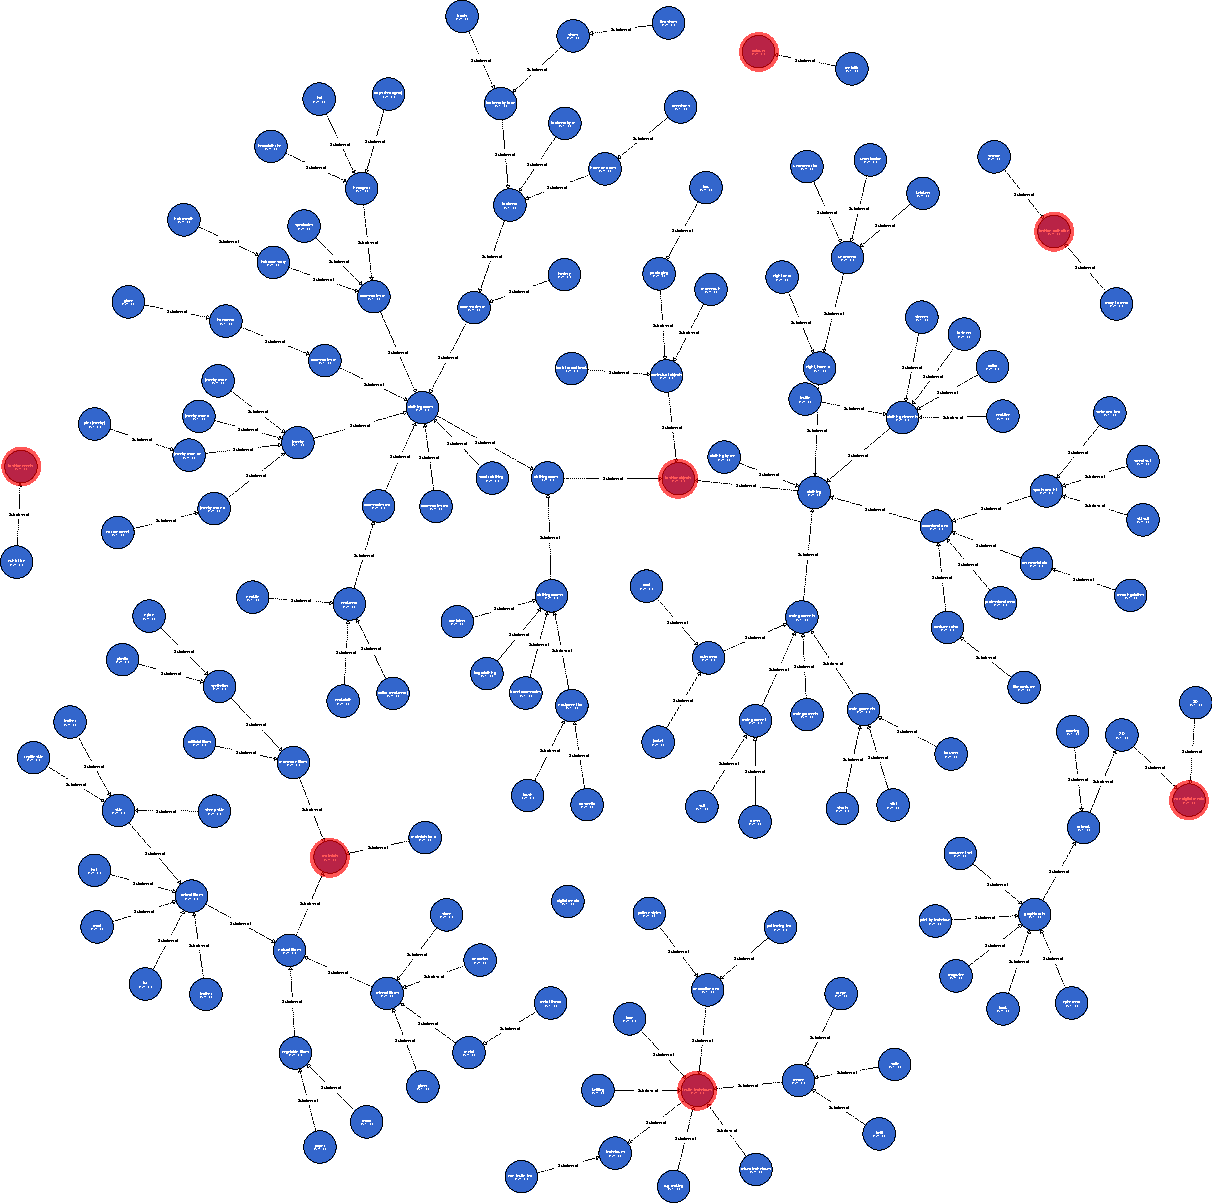
\includegraphics[width=\textwidth]{Picture/europeana_tree.pdf}
	 \caption[Caption for LOF]{grafo ontologia \texttt{europeana}\footnotemark}
\end{figure}
\footnotetext{Il grafo non è completo, le sottoclassi sono troppe per ottenere un'immagine leggibile, WebVOWL permette di far collassare le classi operando una sorta di taglio in profondità del grafo}
Nel capitolo \ref{ch4} abbiamo riportato la struttura dell'ontologia con le nuove relazioni definite su essa (figura \ref{fig:ontEur}).

\section{In Protégé}
Provando a editare il tesauro in Protégé, vediamo che vengono riconosciute come classi quella dei \verb|Concepts| e quella dei \verb|ConceptScheme|, tutti gli elementi del tesauro sono individui. In particolare i concetti fondamentali appartengono alla classe \verb|ConceptScheme|, tutti gli altri alla classe \verb|Concept|. Tra gli strumenti base di refactor di Protégé non ve ne sono per trasformare degli individui in classi, tanto meno mantenendo la struttura gerarchica specificata nel tesauro; non teniamo conto dei plug-in che permettono di scrivere programmi, ad esempio in java\footnote{\url{https://www.java.com/}}, per operare delle trasformazioni simili a quelle fatte con \cduce. Senza voler operare in modo puntuale su ogni individuo per trasformarlo manualmente in una classe, ciò che si può fare è comunque definire le stesse relazioni che abbiamo accennato nel paragrafo precedente (\ref{expr}), che avranno in questo caso dominio e range coincidenti (individui di classe \verb|Concepts|). In questo modo possiamo comunque aumentare l'espressività del tesauro, ma con due grandi vincoli:
\begin{itemize}
	\item non avremo il supporto dei reasoner per verificare la correttezza delle relazioni che valorizzeremo (ad esempio: siccome dominio e range della relazione \say{è fatto di} sono la stessa classe, potremo liberamente creare la relazione: \say{velluto è fatto di allumino});
	\item se volessimo definire delle relazioni di sottogenere più complesse, dovremo farlo tramite la definizione di relazioni, anziché con la più naturale definizione di sottoclasse.
\end{itemize}
\section{Conclusioni}
Nel contesto della re-ingegnerizzazione di un tesauro, \cduce si dimostra molto più versatile di Protégé, questo è dovuto principalmente a due fattori:
\begin{itemize}
	\item come si legge in \cite{re_engineeringThesaurus}, una parte importante del processo di trasformazione è la conversione sintattica dei tag, in questo \cduce è uno strumento molto efficace;
	\item Protégé è uno strumento per editare ontologie espresse in OWL \cite{protege_doc} e, nonostante sia molto potente e versatile, non è lo strumento più indicato per operare su un tesauro.
\end{itemize}
In questo frangente, l'uso di un linguaggio di programmazione che ci permettesse di definire esattamente come manipolare i dati è stato essenziale per ottenere un buon risultato di traduzione. Una volta acquisite delle competenze di base abbastanza solide con \cduce e avendo familiarità con gli strumenti che mette a disposizione, la scrittura di un programma che esegue la traduzione da tesauro a ontologia non risulta particolarmente complessa o lunga in termini di tempo (come testimonia la funzione del listato \ref{lst:refactor_compact}).

Dal punto di vista funzionale, abbiamo sfruttato la possibilità di definire funzioni avendo un sofisticato controllo sul tipo delle espressioni che stavamo trattando; questo ha permesso di evitare subito degli errori che, con linguaggi imperativi, non sarebbero emersi fino al momento dell'esecuzione. In particolare dovendo lavorare alternativamente su liste ed elementi singoli è capitato spesso che il tipo inferito fosse una lista, mentre il tipo richiesto fosse un elemento o viceversa (in un linguaggio come C, con l'uso di vettori e puntatori, un errore del genere avrebbe potenzialmente richiesto molto tempo per essere individuato e risolto).